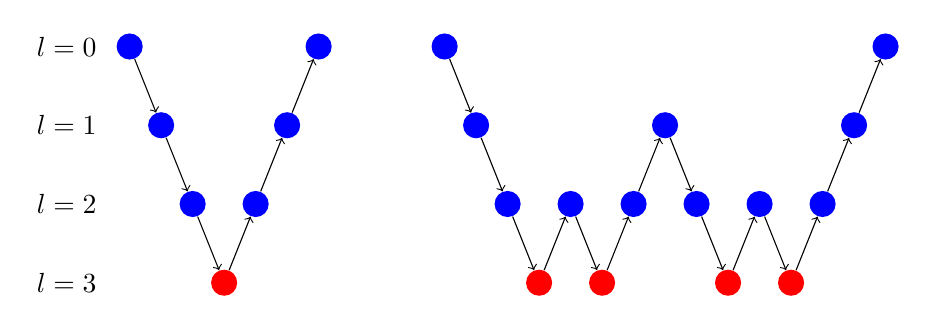
\begin{tikzpicture}

 \begin{scope}[xscale=2/5]

  \node (sh) at (-5,3) { $l=0$ };
  \node (shh) at (-5,2) { $l=1$ };
  \node (shhh) at (-5,1) { $l=2$ };
  \node (shhhh) at (-5,0) { $l=3$};

  %\node (title) at (0,5) { V-cycle k=1};
  %\node (title2) at (14,5) {W-cycle k=2};

    \node[circle,fill=blue] (a) at (-3,3) { };
    \node[circle,fill=blue] (b) at (-2,2) {};
    \node[circle,fill=blue] (c) at (-1,1) {};
    \node[circle,fill=red] (d) at (0,0) {};
    \node[circle,fill=blue] (e) at (1,1) {};
    \node[circle,fill=blue] (f) at (2,2) {};
    \node[circle,fill=blue] (g) at (3,3) {};

    \draw[->] (a) -- (b);
    \draw[->] (b) -- (c);
    \draw[->] (c) -- (d);
    \draw[->] (d) -- (e);
    \draw[->] (e) -- (f);
    \draw[->] (f) -- (g);

    \node[circle,fill=blue] (aa) at (7,3) { };
    \node[circle,fill=blue] (ab) at (8,2) {};
    \node[circle,fill=blue] (ac) at (9,1) {};
    \node[circle,fill=red] (ad) at (10,0) {};
    \node[circle,fill=blue] (ae) at (11,1) {};
    \node[circle,fill=red] (af) at (12,0) {};
    \node[circle,fill=blue] (ag) at (13,1) {};
    \node[circle,fill=blue] (ah) at (14,2) {};
    \node[circle,fill=blue] (ai) at (15,1) {};
    \node[circle,fill=red] (aj) at (16,0) {};
    \node[circle,fill=blue] (ak) at (17,1) {};
    \node[circle,fill=red] (al) at (18,0) {};
    \node[circle,fill=blue] (am) at (19,1) {};
    \node[circle,fill=blue] (an) at (20,2) {};
    \node[circle,fill=blue] (ao) at (21,3) {};

    \draw[->] (aa) -- (ab);
    \draw[->] (ab) -- (ac);
    \draw[->] (ac) -- (ad);
    \draw[->] (ad) -- (ae);
    \draw[->] (ae) -- (af);
    \draw[->] (af) -- (ag);
    \draw[->] (ag) -- (ah);
    \draw[->] (ah) -- (ai);
    \draw[->] (ai) -- (aj);
    \draw[->] (aj) -- (ak);
    \draw[->] (ak) -- (al);
    \draw[->] (al) -- (am);
    \draw[->] (am) -- (an);
    \draw[->] (an) -- (ao);

 \end{scope}

\end{tikzpicture}

